\documentclass{beamer}

\usepackage[T1]{fontenc} 
\usepackage[latin1]{inputenc}
%% \usepackage[frenchb]{babel}

\usetheme{Warsaw}

% Supprimer les icones de navigation (pour les transparents)
\setbeamertemplate{navigation symbols}{}

\usepackage{tikz}
\usetikzlibrary{decorations, decorations.pathreplacing, decorations.pathmorphing, shapes}

\title[Les Bases de la Biologie]{Pr{\'e}sentation pour "d{\'e}butants"\\Les Bases de la Biologie}
\author{Gabriel Chandesris}
%% \institute{ --- }
\institute{ 
\includegraphics[height=0.5cm]{img/logo_glider.png} }
%% \logo{ 
\includegraphics[height=2.5cm]{img/logo_glider.png} }

\date{\today}

\begin{document}

\begin{frame}
	\titlepage
\end{frame}

\begin{frame}
	\frametitle{Contenu de cette pr{\'e}sentation}
	\small \tableofcontents[hideallsubsections]
\end{frame} 

%%%%% %%%%% %%%%% %%%%% %%%%% Partie I %%%%% %%%%% %%%%% %%%%% %%%%% 

%% \section{Le Vif du sujet}
%% \begin{frame}
%% 	\frametitle{Le Vif du sujet}
%% 	\tableofcontents[sections=1,currentsection,subsectionstyle=show/shaded/hide] %% sectionstyle=hide/hide,
%% \end{frame} 

\section{Cellules, types cellulaires et ...}
\begin{frame}
	\frametitle{Cellules, types cellulaires et ...}
	\tableofcontents[sections=1,currentsection,subsectionstyle=show/shaded/hide]
\end{frame} 

\subsection{"Types Cellulaires"}
\begin{frame}
	\frametitle{"Types Cellulaires"}
	\begin{itemize}
		\item Bact{\'e}ries / Arch{\'e}bact{\'e}ries (membranes et "m{\'e}lange interne") ; 
		\item Eukaryotes (membranes, organites, sous-parties, 
		\begin{itemize}
			\item Noyau (principale localisation du g{\'e}nome), Appareil de Golgi, Cytosquelette, v{\'e}sicules diverses...
			\item Plantes : Chloroplastes (interaction lumi{\`e}re-mati{\`e}re, g{\'e}nome sp{\'e}cifique pour certains constituants) ; 
			\item Animaux : Mitochondries (g{\'e}nome sp{\'e}cifique pour certains constituants) ; 
		\end{itemize}
		\item Virus : "organismes incomplets", classification particuli{\`e}re (selon ADN, ARN, cellules-cibles, activit{\'e}, capside, chargement...). 
	\end{itemize}
\end{frame}

\subsection{Fonctionnement Cellulaire}
\begin{frame}
	\frametitle{ Fonctionnement Cellulaire }
	\tableofcontents[sections=1,currentsection,subsectionstyle=show/shaded/hide]
\end{frame} 

\subsubsection{ Membranes cellulaires }
\begin{frame}
	\frametitle{ Membranes cellulaires }
	\begin{itemize}
		\item Isolement ; 
		\item Canaux (Ioniques, Transferts de mol{\'e}cules complexes, ...) ; 
		\item Organites : subdivision de l'espace par fonctions (?!) ; 
		\item ... 
		\item ... 
	\end{itemize}
\end{frame}

\subsubsection{ Enzymes et activit{\'e}s catalytiques }
\begin{frame}
	\frametitle{ Enzymes et activit{\'e}s catalytiques }
	\begin{itemize}
		\item element 1
		\item element 2
		\item element 3
	\end{itemize}
\end{frame}

\subsubsection{ Structures }
\begin{frame}
	\frametitle{ Structures }
	\begin{itemize}
		\item element 1
		\item element 2
		\item element 3
	\end{itemize}
\end{frame}

%%%%% %%%%% %%%%% %%%%% %%%%% PARTIE II %%%%% %%%%% %%%%% %%%%% %%%%% 

\section{Dogme central de la Biologie (DCB)}
\begin{frame}
	\frametitle{Dogme central de la Biologie (DCB)}
	\tableofcontents[sections=2,currentsection,subsectionstyle=show/shaded/hide]
\end{frame} 

\subsection{Dogme central de la Biologie (DCB) : d{\'e}finition}
\begin{frame}
	\frametitle{Dogme central de la Biologie (DCB) : d{\'e}finition}
	\begin{itemize}
		\item Nom r{\'e}el : "Th{\'e}orie Fondamentale de la biologie Mol{\'e}culaire", Francis Crick en 1958 : \texttt{central dogma of molecular biology}, transform{\'e} et confirm{\'e} par la suite ; 
		\item En r{\'e}sum{\'e} : \texttt{L'ADN dirige sa propre r{\'e}plication en ADN identique, ainsi que sa transcription en ARN, pouvant ou non {\^e}tre traduit en prot{\'e}ines}
		\item Hypoth{\`e}ses, {\'e}volution, ajouts {\`a} la compr{\'e}hension (sans forc{\'e}ment de remise en cause fondamentale). 
	\end{itemize}
\end{frame}

\subsection{Dogme central de la Biologie (DCB) : "version 1.0"}
\begin{frame}
	\frametitle{Dogme central de la Biologie (DCB) : "version 1.0"}
	
	\begin{minipage}[ht]{0.50\linewidth}
	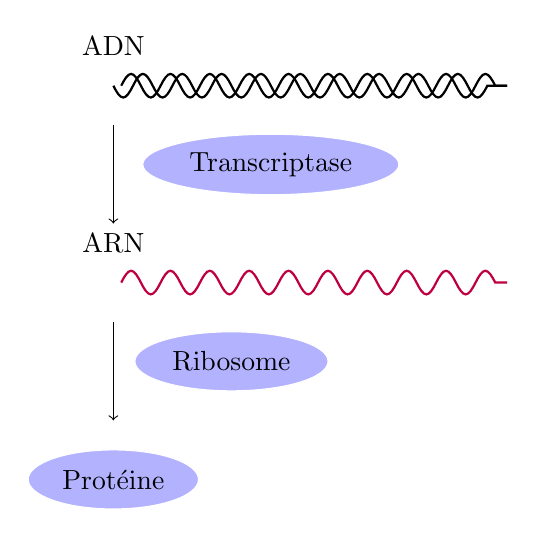
\begin{tikzpicture}[decoration={coil},
		dna/.style={decorate, thick, decoration={aspect=0, segment length=0.5cm}},
		protein/.style={ellipse, draw=white, minimum width=1cm, minimum height=1cm}]
		
		%% DNA
		\draw[dna, decoration={amplitude=.15cm}] (.1,0) -- (5,0);
		\draw[dna, decoration={amplitude=-.15cm}] (0,0) -- (5,0);
		\node at (0,0.5) {ADN};
		
		\draw [->] (0,-0.50) -- (0,-1.75);
		\node [protein, minimum height=.75cm,fill=blue!30] at (2.0,-1.0) {Transcriptase};
		
		%% RNA
		\draw[dna, decoration={amplitude=.15cm}, color=purple] (.1,-2.5) -- (5,-2.5);
		\node at (0,-2.0) {ARN};
		
		\draw [->] (0,-3) -- (0,-4.25);
		\node [protein, minimum height=.75cm,fill=blue!30] at (1.5,-3.5) {Ribosome};
	
		%% Protein
		\node [protein, minimum height=.75cm,fill=blue!30] at (0,-5.0) {Prot{\'e}ine};
	\end{tikzpicture}
	\end{minipage} \hfill \begin{minipage}[ht]{0.45\linewidth}
		\begin{itemize}
			\item ADN : Bases Nucl{\'e}iques (A, C, G et T)~\\~\\~\\
			\item ARN : Bases Nucl{\'e}iques (A, C, G et U)~\\~\\~\\
			\item Prot{\'e}ine : Acides Amin{\'e}s (20, cf. nomenclature)
		\end{itemize}
	\end{minipage} 

\end{frame}

\subsection{Dogme central de la Biologie (DCB) : "version 2.0"}
\begin{frame}
	\frametitle{Dogme central de la Biologie (DCB) : "version 2.0"}

	\begin{minipage}[ht]{0.50\linewidth}
	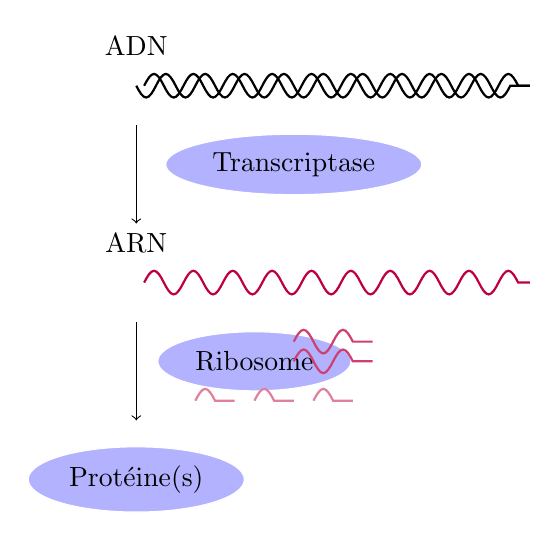
\begin{tikzpicture}[decoration={coil},
		dna/.style={decorate, thick, decoration={aspect=0, segment length=0.5cm}},
		protein/.style={ellipse, draw=white, minimum width=1cm, minimum height=1cm}]
		
		%% DNA
		\draw[dna, decoration={amplitude=.15cm}] (.1,0) -- (5,0);
		\draw[dna, decoration={amplitude=-.15cm}] (0,0) -- (5,0);
		\node at (0,0.5) {ADN};
		
		\draw [->] (0,-0.50) -- (0,-1.75);
		\node [protein, minimum height=.75cm,fill=blue!30] at (2.0,-1.0) {Transcriptase};
		
		%% RNA
		\draw[dna, decoration={amplitude=.15cm}, color=purple] (.1,-2.5) -- (5,-2.5);
		\node at (0,-2.0) {ARN};
		
		\draw [->] (0,-3) -- (0,-4.25);
		\node [protein, minimum height=.75cm,fill=blue!30] at (1.5,-3.5) {Ribosome};
		\draw[dna, decoration={amplitude=.15cm}, color=purple!75] (2,-3.25) -- (3,-3.25);
		\draw[dna, decoration={amplitude=.15cm}, color=purple!75] (2,-3.50) -- (3,-3.50);
		\draw[dna, decoration={amplitude=.15cm}, color=purple!50] (0.75,-4) -- (1.25,-4);
		\draw[dna, decoration={amplitude=.15cm}, color=purple!50] (1.50,-4) -- (2.00,-4);
		\draw[dna, decoration={amplitude=.15cm}, color=purple!50] (2.25,-4) -- (2.75,-4);
	
		%% Protein
		\node [protein, minimum height=.75cm,fill=blue!30] at (0,-5.0) {Prot{\'e}ine(s)};
	\end{tikzpicture}
	\end{minipage} \hfill \begin{minipage}[ht]{0.45\linewidth}
		\begin{itemize}
			\item ARNm (messager)
			\item ARNr (ribosomal)
			\item ARNt (transfert)
			\item {\'E}pissage alternatif (du fait de l'existence des introns et des exons : un seul ARNm issu du m{\^e}me g{\`e}ne peut donner plusieurs prot{\'e}ines chez les eukaryotes).
		\end{itemize}
	\end{minipage} 

\end{frame}

\subsection{Dogme central de la Biologie (DCB) : "version 3.0"}
\begin{frame}
	\frametitle{Dogme central de la Biologie (DCB) : "version 3.0"}
	\begin{itemize}
		\item ARNnc (dont ARNi) / ARN interf{\'e}ron ; 
		\item {\'E}pig{\'e}n{\'e}tique ; 
		\item R{\'e}gulation interne de l'expression du g{\'e}nome ; 
		\item ... 
		\item ... 
	\end{itemize}
\end{frame}

%%%%% %%%%% %%%%% %%%%% %%%%% PARTIE III %%%%% %%%%% %%%%% %%%%% %%%%% 

\section{Grands types de mol{\'e}cules}
\begin{frame}
	\frametitle{Grands types de mol{\'e}cules}
	\tableofcontents[sections=3,currentsection,subsectionstyle=show/shaded/hide]
\end{frame} 

\subsection{ Glucides }
\begin{frame}
	\frametitle{ Glucides }
	\begin{itemize}
		\item element 1
		\item element 2
		\item element 3
	\end{itemize}
\end{frame}

% Define decoration
\pgfdeclaredecoration{lipidleaflet}{initial}
{
  % Place as many segments as possible along the path to decorate
  % the minimum distance between two segments is set to 7 pt.
  \state{initial}[width=\pgfdecoratedpathlength/floor(\pgfdecoratedpathlength/7pt)]
  {
    % Draw the two acyl chains
    \pgfpathmoveto{\pgfpoint{-1pt}{0pt}}
    \pgfpathlineto{\pgfpoint{-1pt}{-10pt}}
    \pgfpathmoveto{\pgfpoint{1pt}{0pt}}
    \pgfpathlineto{\pgfpoint{1pt}{-10pt}}
    % Draw the head group
    \pgfpathmoveto{\pgfpoint{1pt}{0pt}}
    \pgfpathcircle{\pgfpoint{0pt}{2pt}}{2.5pt}
  }
  \state{final}
  {
    \pgfpathmoveto{\pgfpointdecoratedpathlast}
  }
}

\subsection{ Lipides }
\begin{frame}
	\frametitle{ Lipides }
	\begin{minipage}[ht]{0.50\linewidth}
		\begin{itemize}
			\item element 1
			\item element 2
			\item element 3
		\end{itemize}
	\end{minipage} \hfill \begin{minipage}[ht]{0.45\linewidth}
		% Draw a vesicle composed of two lipid layers
		\begin{tikzpicture}[scale=0.65]
			% Micelle
			\draw[decorate, decoration={lipidleaflet, mirror}] (0, 3) circle (0.6cm);
			\draw (0, 2) node {Micelle};
			
			% Inverted micelle
			\draw[decorate, decoration={lipidleaflet}] (0, 0) circle (0.45cm);
			\draw (0, -1) node {Inverted micelle};
			
			% Lipid bilayer
			\draw[decorate, decoration={lipidleaflet, mirror}]
			  (-1, -2.8) -- (2, -2.8);
			\draw[decorate, decoration={lipidleaflet}]
			  (-1, -2) -- (2, -2);
			\draw (0, -3.5) node {Lipid bilayer};
			
			% Vesicle
			\draw[decorate, decoration={lipidleaflet}] (5, 0.5) circle (2.5cm);
			\draw[decorate, decoration={lipidleaflet, mirror}] (5, 0.5) circle (3.3cm);
			\draw (5, -3.5) node {Vesicle};
		\end{tikzpicture}
	\end{minipage}
\end{frame}

\subsection{ Prot{\'e}ines }
\begin{frame}
	\frametitle{ Prot{\'e}ines }
	\begin{itemize}
		\item Polym{\`e}res d'Acides Amin{\'e}s ; 
		\item Activit{\'e}s diverses : catalytique, structurale...
		\item ... 
	\end{itemize}
\end{frame}

%%%%% %%%%% %%%%% %%%%% %%%%% PARTIE IV %%%%% %%%%% %%%%% %%%%% %%%%% 

\section{Information g{\'e}n{\'e}tique }
\begin{frame}
	\frametitle{Information g{\'e}n{\'e}tique }
	\tableofcontents[sections=4,currentsection,subsectionstyle=show/shaded/hide]
\end{frame} 

\subsection{ ADN et ARN }
\begin{frame}
	\frametitle{ ADN et ARN }
	\begin{itemize}
		\item ADN bicat{\'e}naire ; 
		\item ARN monocat{\'e}naire ; 
		\item activit{\'e} catalytique des ARN ; 
	\end{itemize}
\end{frame}

\subsection{ Mutations et autres changements }
\begin{frame}
	\frametitle{ Mutations et autres changements }
	\begin{itemize}
		\item mutation : substitution, deletion, insertion ; 
		\item transposition / r{\'e}trotransposition (insertion de g{\`e}nes viraux et d{\'e}placements sur le g{\'e}nome) ; 
		\item d{\'e}tournements viraux (et autres parasites) : int{\'e}r{\^e}ts aussi ; 
	\end{itemize}
\end{frame}

\subsection{ G{\'e}nomique / M{\'e}ta-G{\'e}nomique }
\begin{frame}
	\frametitle{ G{\'e}nomique / M{\'e}ta-G{\'e}nomique }
	\begin{itemize}
		\item Une cellule avec un seul g{\'e}nome (noyau cellulaire + organites : mitochondries / chloroplastes) ; 
		\item Cellules sp{\'e}cialis{\'e}es au sein d'un organisme (tissus sp{\'e}cialis{\'e}s) ; 
		\item Groupement de bact{\'e}ries qui croissent ensemble au sein d'un m{\^e}me environnement (et chacune au g{\'e}nome "incomplet") ; 
	\end{itemize}
\end{frame}

\subsection{ Esp{\`e}ce(s) : une d{\'e}finition ? }
\begin{frame}
	\frametitle{ Esp{\`e}ce(s) : une d{\'e}finition ? }
	\begin{itemize}
		\item element 1
		\item element 2
		\item element 3
	\end{itemize}
\end{frame}

%%%%% %%%%% %%%%% %%%%% %%%%% PARTIE V %%%%% %%%%% %%%%% %%%%% %%%%% 

\section{Darwinisme, N{\'e}odarwinisme et s{\'e}lection naturelle }
\begin{frame}
	\frametitle{Darwinisme, N{\'e}odarwinisme et s{\'e}lection naturelle }
	\tableofcontents[sections=5,currentsection,subsectionstyle=show/shaded/hide]
\end{frame} 

\subsection{ Darwinisme, N{\'e}odarwinisme et s{\'e}lection naturelle }
\begin{frame}
	\frametitle{ Darwinisme, N{\'e}odarwinisme et s{\'e}lection naturelle }
	\begin{itemize}
		\item \emph{d{\'e}finitions {\`a} pr{\'e}ciser} ; 
		\item "la mutation pr{\'e}c{\`e}de la s{\'e}lection", ... ; 
		\item "survie du plus apte / adaptable dans un environnement donn{\'e}, et non du plus fort" ; 
		\item conservation de maladies g{\'e}n{\'e}tiques / diversit{\'e} g{\'e}n{\'e}tique ; 
		\item divergence {\'e}volutive visible, et {\'e}galement convergence {\'e}volutive (vision, pattes, ailes...) ; 
		\item \textsc{Reine Rouge} ({\'e}volution permanente li{\'e}e aux changements permanents) et \textsc{Fou Du Roi} (saut {\'e}volutifs / forte p{\'e}riode de s{\'e}lection lors d'un fort changement environnemental)
		\item[] 
		\item \texttt{https://fr.wikipedia.org/wiki/Cat{\'e}gorie:Th{\'e}orie\_sur\_l'{\'e}volution} (Fixisme, neutre, Lamarck...)
	\end{itemize}
\end{frame}

%%%%% %%%%% %%%%% %%%%% %%%%% PARTIE VI %%%%% %%%%% %%%%% %%%%% %%%%% 

\section{Int{\'e}r{\^e}ts techniques / technologiques }
\begin{frame}
	\frametitle{Int{\'e}r{\^e}ts techniques / technologiques }
	\tableofcontents[sections=6,currentsection,subsectionstyle=show/shaded/hide]
\end{frame} 

\subsection{ Int{\'e}r{\^e}ts techniques / technologiques (1)  }
\begin{frame}
	\frametitle{ Int{\'e}r{\^e}ts techniques / technologiques (1) }
	\begin{itemize}
		\item S{\'e}lection de lign{\'e}es (souris, bact{\'e}ries, levures, champignons...) sur des crit{\`e}res int{\'e}ressants / crit{\`e}res d'int{\'e}r{\^e}t ; 
		\item Insertions et / ou modifications g{\'e}n{\'e}tiques de bact{\'e}ries ou d'eukaryotes (phages / virus, plasmides, CRISPR-Cas9...) ; 
		\item Combinaison / fusion cellulaire (par exemple pour la production d'anticorps monoclonaux) ; 
		\item ... 
	\end{itemize}
\end{frame}

\subsection{ Int{\'e}r{\^e}ts techniques / technologiques (2) }
\begin{frame}
	\frametitle{ Int{\'e}r{\^e}ts techniques / technologiques (2) }
	\begin{itemize}
		\item D{\'e}tection fine de mol{\'e}cules (amplification type PCR, changement d'activit{\'e} m{\'e}tabolique) ; 
		\item Reproduction / culture / production de mol{\'e}cules d'int{\'e}r{\^e}t (en fermenteur, avec fixation sur support) : plus facile car performance catalytique biologique {\`a} temp{\'e}rature ambiante (m{\'e}dicaments, mol{\'e}cules nutritives, vitamines) ;  
		\item Usage dans le recyclage {\'e}galement : transformation d'{\'e}l{\'e}ments toxiques et / ou d{\'e}chets) ;
		\item ... 
	\end{itemize}
\end{frame}

\subsection{ Lire et {\'E}crire de l'Information G{\'e}n{\'e}tique }
\begin{frame}
	\frametitle{ Lire et {\'E}crire de l'Information G{\'e}n{\'e}tique }
	\begin{itemize}
		\item Lecture : S{\'e}quen\c{c}age d'Acides Nucl{\'e}iques (ShotGun et autres m{\'e}thodes, Amorces pour PCR et autres, r{\'e}f{\'e}rences {\`a} (re)trouver)
		\item {\'E}criture : Synth{\`e}se d'Acides Nucl{\'e}iques (r{\'e}f{\'e}rences : ???)
		\item Stockage de donn{\'e}es ({\'E}criture et Lecture, peristance) \newline
			https://theconversation.com/ladn-sera-t-il-lavenir-du-stockage-de-donnees-159387
		\item ... 
		\item ... 
	\end{itemize}
\end{frame}

%%%%% %%%%% %%%%% %%%%% %%%%% BIBLIOGRAPHIE %%%%% %%%%% %%%%% %%%%% %%%%% 

\def\sectionPartBibliographie{Bibliographie / Mediagraphie}
\section{\sectionPartBibliographie}
\begin{frame}[allowframebreaks]
	\frametitle{\sectionPartBibliographie}
	\nocite{*}
	%\footnotesize
	%toutes references biblio : 6 lettres + 2 chiffres
	\bibliography{presentationBasesBiologie}
	% \bibliographystyle{frplain} % plain or frplain
	\bibliographystyle{plain}
\end{frame}

\end{document}
